\section{DIP开发者激励协议}
\label{sec:dip}

在星云链中,我们提出面向智能合约开发者的DIP(Developer Incentive Protocol,开发者激励协议),周期性对星云链生态中所有智能合约的价值做评估,通过星云币的奖励来感谢为生态助力的优秀开发者。

DIP的设计借助周活跃用户价值总和的概念,每周进行一次,和Nebulas Rank计算周期一致。对于智能合约C,假设本周活跃账户地址集合为WAA(Weekly Active Addresses),其中根据\refsec{sec:nrrank}的Nebulas Rank分数,计算周活跃地址的NR之和作为合约C的贡献值SCS(Smart Contract Score)。

\begin{align}
SCS(C)=\sum_{addr \in WAA}NR(addr)
\end{align}

每周贡献值SCS得到智能合约贡献度排名SCR(Smart Contract Rank),取Top N的智能合约,它们对应的开发者将按比例瓜分M个星云币作为奖励,为了避免恶意刷榜,DIP的分配曲线被设计得较为平均,如图\ref{fig:dip}所示,但依旧保证Top 1的收益为Top N收益的一倍以示贡献度大小的区别,如公式\ref{formula:dip}所示。

\begin{alignat}{2}
Coin(C) = & \quad kln(N+1-SCR(C))+b \label{formula:dip} \\
\mbox{s.t.}\quad & kln(N) + b = 2b \nonumber \\
& \sum_{x=1}^{N}(kln(x) + b) = M \nonumber
\end{alignat}

\begin{figure}[h] 
\centering
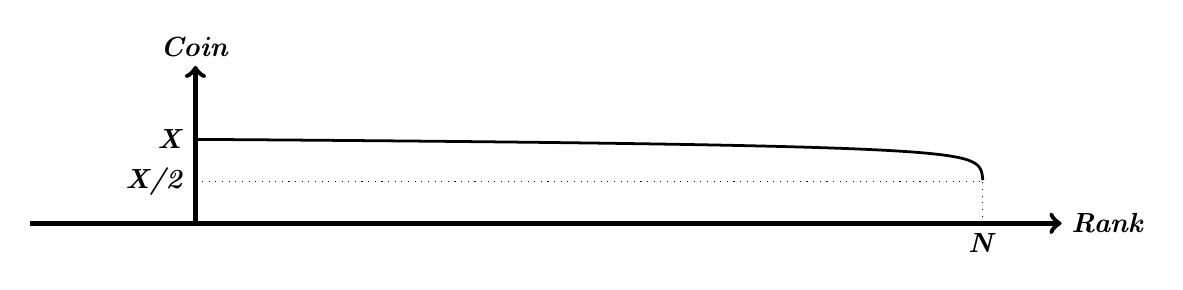
\begin{tikzpicture}
\coordinate (OR) at (0.00, 0.00);
\coordinate (LX) at (-2.10, 0.00); % left x
\coordinate (RX) at (11.00, 0.00); % right x
\coordinate (BY) at (0.00, 0.00); % bottom y
\coordinate (TY) at (0.00, 2.00); % top y
\draw[->][line width=1.75pt] (LX) -- (RX);
\node[right,black] at (11,0) {\textbf{\textit{Rank}}};
\draw[->][line width=1.75pt] (BY) -- (TY);
\node[above,black] at (0, 2) {\textbf{\textit{Coin}}};
\draw[dotted] (0,0.533210267)--(10,0.533210267);
\draw[dotted] (10,0)--(10,0.533210267);
\node[below,black] at (10, 0) {\textbf{\textit{N}}};
\node[left,black] at (0, 0.533210267) {\textbf{\textit{X/2}}};
\node[left,black] at (0, 1.066420536) {\textbf{\textit{X}}};
\draw[black, line width=1.00pt, domain=0:10.00,samples=3000] plot[smooth](\x, {.066598275 * ln(3001-\x * 300) + .533210267});

\end{tikzpicture}
\label{fig:dip}
\caption{DIP奖励分配曲线}
\end{figure}

为了鼓励星云链生态智能合约的多样性,DIP规定每个智能合约同一个版本最多可以接受K次奖励,当使用星云原力对合约做版本更新后,新版本将可以再次接受最多K次奖励。

DIP的奖励将会由各个节点单独计算发放,假设星云链平均每S秒出一个区块,那么每隔24*7*3600/S个区块,所有节点将会计算一次DIP的奖励,并且发给对应的智能合约的提币地址中。
